\chapter{Introduction}
\label{ch:intro}
In the 1790s, John Michell of England and Pierre-Simon Laplace of France 
independently imagined an ``invisible star'', 
an object whose escape velocity is greater than the speed of light, 
and they both used Newton's gravitational laws to calculate the mass and size of such object \citep{montgomery2009}.  \\

A century ago, in \citeyear{einstein1915}, Albert Einstein completed his General theory of Relativity 
and submitted to the Prussian Academy of Sciences a seminal paper 
where he published the full treatment of his ``field equations''. 
Einstein's theory finally explained the anomalous precession of the perihelion of Mercury, 
and predicted the deflection of light by means of gravitational fields 
and the gravitational redshift of light. 
Albert Einstein willingly embraced these three implications of his theoretical work, 
and was confident about a timely verification of the last two. 
However, he never accepted nor demonstrated any interest in another conclusion of General Relativity, 
i.e.~the existence of regions of the space-time where the force of gravity is so strong 
that not even light can escape. 
Ironically, while some of his colleagues were fascinated by these exotic, dark objects -- 
first of all the American physicist John Archibald Wheeler, who coined and popularised the term ``black hole'' -- 
Einstein strongly opposed and fought against the idea of those weird mathematical singularities for all his life 
\citep{thorne1994}. 
In his \citeyear{einstein1939} article, 
Einstein derived the relativistic equations that describe a stationary cluster of particles 
orbiting on the surface of a sphere. 
He imagined to gradually reduce the radius of the sphere, 
forcing the particles to move faster and faster, 
and demonstrated that the velocity of the particles was reaching the speed of light 
before the cluster was small enough to become a black hole. 
Einstein interpreted his calculations as a proof of the fact that black holes cannot exist. 
He concluded the article writing ``The essential result of this investigation is a clear understanding as to why 
the Schwarzschild singularities do not exist in physical reality. [...] 
The Schwarzschild singularity does not appear for the reason that matter cannot be concentrated arbitrarily''.  \\

Today, not only their existence is unanimously taken for granted by the scientific community, 
but black holes are at the centre of some of the most active research fields of astronomy. 
We know that they come in different flavours and they occupy a wide range of masses, 
going from the hypothetical, minuscule, primordial black holes (e.g.~\citealt{carrhawking1974}), 
generated by density fluctuations of matter during the very first moments of the Universe's expansion 
after the Big Bang, 
through the well understood stellar black holes (e.g.~\citealt{shahbaz1999}), 
remnant products left behind after the death of a massive star, 
to the so called ``massive black holes'', 
occupying the centre of nuclear star clusters and galaxies. 
Massive black holes are further differentiated into two classes according to their mass: 
Intermediate Mass Black Holes (within the mass range $100 - 10^5~\rm M_\odot$, e.g.~\citealt{millercolbert2004,vandermarel2004}), 
still lacking many incontrovertible direct detections 
(but for which we might accumulate evidence over the next years, e.g.~\citealt{pasham2014}), 
and Supermassive Black Holes (e.g.~\citealt{ferrarese2006book}), 
which are the focus of this thesis. 


\section{Supermassive black holes} 
An astrophysical black hole is a region of the space-time whose escape velocity is greater than the speed of light.
Black holes are the simplest objects in the Universe. 
They are completely characterised by three properties: mass, spin (or angular momentum) and electric charge. \\

Supermassive black holes (SMBHs) are the most massive black holes known, with typical masses  
$M_{\rm BH} \approx 10^6 - 10^9~\rm M_{\odot}$.
This class of black holes was first theorised \citep{lynden-bell1969,wolfeburbidge1970} after the discovery of quasars.
Quasars can be as luminous as galaxies ($\approx 10^{46}~\rm erg~s^{-1}$).
However, their rapid variability ($\approx$ minutes) at high energies implies tiny sizes for these objects 
($\approx 10^{-6}~\rm pc$), even smaller than the Solar System.
Small sizes and powerful energy outputs led to the conclusion that accreting SMBHs are the engine of quasars
\citep{salpeter1964,zeldovichnovikov1964,lynden-bell1978}. \\

Because quasars were numerous at high redshift, the Universe should be populated with relic black holes \citep{soltan1982}. 
Assuming that the luminosity of quasars is produced by accretion of mass onto the central black hole, 
Andrzej Soltan calculated a lower limit for the integrated energy density due to quasar light, 
derived the corresponding value of mass density of accreted material, 
and showed that, because this mass must be discretely distributed in today's Universe, 
then most, if not all, nearby galaxies host quiescent black holes in their nuclei, 
each black hole having a mass in the $10^8 - 10^9~\rm M_{\odot}$ range. 
This realisation motivated the search of SMBHs at the centre of galaxies, 
i.e.~at the bottom of the potential well, 
where dynamical friction is expected to drag compact massive objects. \\

The gravitational potential of a SMBH dominates over the gravitational potential of the host galaxy within the 
sphere-of-influence radius 
\begin{equation}
r_{\rm h} = \frac{G M_{\rm BH}}{\sigma_*^2} \approx 0.45 \biggl ( \frac{M_{\rm BH}}{10^6 \rm~M_{\odot}} \biggr ) 
\biggl ( \frac{100 \rm~km~s^{-1}}{\sigma_*} \biggr ) \rm~pc ,
\end{equation}
where $G$ is the gravitational constant and $\sigma_*$ is the velocity dispersion of the stars in the 
host galaxy's bulge.
A dynamical detection of a black hole requires the ability to resolve its sphere-of-influence.
For local galaxies ($\lesssim 20~\rm Mpc$), it demands a subarcsecond spatial resolution.
It is only after the introduction of CCD on spectrographs ('80s) that stellar dynamical 
detections of black holes became possible (see the references in the reviews by 
\citealt{kormendyrichstone1995} and \citealt{richstone1998}).
The number of dynamical black hole mass measurements has increased with time and it has recently become a 
statistically meaningful sample with which one can study SMBH demographics. 
It is now generally accepted that SMBHs reside at the centre of most, if not all, 
massive galaxies, either quiescent or active. 


\subsection{Measuring black hole masses}
Techniques to measure the mass of SMBHs can be divided into two main categories: direct and indirect methods 
(see \citealt{ferrareseford2005} for a thorough review). 
In direct methods, the mass of a black hole is determined from its gravitational imprint 
in the motion of the surrounding stars or gas. 
The spatial resolution of the observing instrument has to be smaller than the size of the black hole sphere-of-influence, 
which implies challenging technology and time-consuming observations. 
In indirect methods, one adopts approximations to the direct methods 
or uses a parameter of the host galaxy as a proxy to infer the black hole mass 
on the basis of observed scaling relations. \\

Sgr A$^*$, the radio source associated with the Galactic black hole, represents a special case study. 
Thanks to its proximity ($8.28 \pm 0.33 \rm~kpc$, \citealt{genzel2010}), 
near infrared techniques have made possible to resolve and follow each individual star 
orbiting around Sgr A$^*$. 
From the analysis of these orbits, 
\citet{ghez2008} derived a best-fit central mass of $(4.5 \pm 0.4) \times 10^6 \rm~M_\odot$. \\

When measuring black hole masses in gas-poor early-type galaxies, 
the primary method of choice is based on modelling the integrated kinematics of stars 
acquired through high spatial resolution spectroscopy. 
Because to a good approximation the stars in a local galaxy constitute a collisionless system, 
it is possible to describe their motion analytically and constrain the central gravitational potential. 
The best-fit model to the observed integrated stellar kinematics 
returns an estimate of the black hole mass and the stellar mass-to-light ratio, 
which are treated as free parameters. 
Although modelling the integrated stellar kinematics can in principle return robust black hole mass estimates, 
this method is not exempted from systematics and degeneracies, 
which are mainly caused by our poor ability to resolve the tiny black hole sphere-of-influence even in the most nearby galaxies 
\citep{valluri2004}. 
\citet{gebhardtthomas2009} first explored the effects of including the additional contribution from a dark matter halo 
when modelling the central stellar kinematics of the galaxy M87.
Their measurement of the black hole mass was over a factor of two larger than previous stellar dynamical measurements 
which did not account for dark matter.  
Upon deriving 10 new black hole mass measurements from the analysis of two-dimensional stellar kinematics, 
\citet{rusli2013bhmassesDM} concluded that the omission of dark matter systematically overestimates the stellar mass-to-light ratio 
and underestimates the black hole mass; 
this bias does not significantly affect the estimate of the black hole mass 
only if the spatial resolution of the observations is at least a factor of 10 smaller 
than the size of the black hole sphere-of-influence.
\citet{merritt2013book} reminds that, 
among all current black hole mass measurements based on stellar-dynamics, 
only three cases were carried out with enough spatial resolution to detect 
a convincing Keplerian rise in the central stellar velocities, 
as expected from the presence of a central massive object. 
From this consideration, he raises doubts about the majority of such black hole mass detections, 
and pessimistically cautions that they should be interpreted as upper limits only. \\

When water maser clouds are present in an Active Galactic Nucleus (AGN) 
in the form of a thin disc (with sub-parsec size) rotating around the central engine 
and heated by the X-ray photons emitted by the AGN accretion disc, 
the gas dynamics can be studied with radio interferometric techniques (e.g.~with the Very Long Baseline Array)
and the central gravitational potential constrained, 
benefiting from a spatial resolution that can be up to $\approx 200$ times higher than that allowed by the Hubble Space Telescope 
(e.g.~the black hole mass measurement in the galaxy NGC 4258, \citealt{miyoshi1995}). 
Water masers allow the most accurate mass measurements for SMBHs in galaxies other than the Milky Way. \\

More than half of massive early-type (elliptical + lenticular) galaxies and virtually all spiral galaxies have 
detectable warm ionised gas in their nuclei \citep{ho1997}, 
whose emission lines are easier to measure than stellar absorption lines. 
In principle, under the assumption that the ionised gas is distributed in a rotationally-supported Keplerian disc, 
where the effects of stellar orbital anisotropy, triaxiality or dark matter are negligible, 
modelling the gas dynamics is conceptually simpler than modelling the integrated stellar kinematics. 
However, as \citet{kormendyho2013} pointed out, unlike stars, gas is subject to non-gravitational perturbations 
(turbulence, shocks, radiation pressure, magnetic fields, etc.), 
hence its dynamics could be much more complicated than the ordered motion assumed within a Keplerian disc model.
\citet{kormendyho2013} compared the common black hole mass measurements obtained from gas and stellar dynamics for eight galaxies 
and concluded that the gas-based measurements are systematically underestimated 
when the modelling of the gas dynamics does not include corrections for large emission-line widths, 
which are speculated to imply significant random motions of gas perturbed by non-gravitational fenomena, such as radio jets. \\

Other black hole mass determination methods can be applied to some AGNs and quasars. 
These techniques rely on fitting accretion disc models to multiwavelength continua spectra \citep{shields1978,malkan1983}
or studying the emission line due to iron fluorescence (e.g.~\citealt{fabian2000,reynoldsnowak2003}).
Reverberation mapping (e.g.~\citealt{peterson1993}) consists of 
modelling the structure of the broad emission-line region of an AGN, 
as probed by the short-term variability of the ionising continuum,
and estimating the black hole mass by assuming a calibration factor that depends on an observed correlation 
between the black hole mass and some host galaxy parameter\footnote{Typically, this scaling factor is calibrated 
on the $M_{\rm BH} - \sigma_*$ relation, i.e.~the observed correlation between black hole mass and host spheroid 
stellar velocity dispersion (e.g.~\citealt{ferraresemerritt2000,gebhardt2000}). }. \\

Building on past catalogs of direct black hole mass measurements 
obtained with stellar-kinematics, gas-dynamics, or water maser techniques, 
\cite{grahamscott2013} compiled a sample of $\approx 80$ galaxies with a reliable measure of $M_{\rm BH}$. 
The galaxy sample used in this work is based on that published by \cite{grahamscott2013}.



\subsection{Scaling relations}
Over the last three decades, observations have demonstrated that 
the black hole mass scales with a number of properties of its host spheroid 
(see Section \ref{sec:spheroid} for the meaning of the term ``spheroid''), 
on scales much larger than the black hole sphere-of-influence.
The black hole mass has been shown to correlate with 
the spheroid luminosity $L_{\rm sph}$ \citep{dressler1989,kormendyrichstone1995}, 
the spheroid stellar velocity dispersion $\sigma_*$ \citep{ferraresemerritt2000,gebhardt2000}, 
the spheroid central radial concentration of stars \citep{graham2001,grahamdriver2007}, 
the spheroid dynamical mass $M_{\rm dyn,sph}$ \citep{magorrian1998,marconihunt2003,haringrix2004}, 
the spheroid gravitational binding energy \citep{allerrichstone2007}, 
the spheroid kinetic energy of random motion \citep{feolimele2005,feolimancini2009},
the spheroid effective radius \citep{sani2011}, 
and the spheroid stellar mass (e.g.~\citealt{magorrian1998,sani2011,beifiori2012,scott2013}).
Other correlations with host galaxy parameters  -- as opposed to spheroid parameters -- have been proposed, such as with
the spiral arm pitch angle \citep{seigar2008,berrier2013}, 
the number of globular clusters \citep{burkerttremaine2010,snyder2011},
the dark matter halo \citep{ferrarese2002}
and the velocity dispersion of the globular clusters \citep{sadouncolin2012,pota2013}. 
Very recently, \cite{lasker2014anal} claimed that the black hole mass correlates equally well with the spheroid and 
the total galaxy luminosity. \\

The astrophysical interest in black hole mass scaling relations can be summarised in three points.
First, the correlations probe a strong connection between SMBHs and their host spheroids.
Exploring how scaling relations have changed throughout the cosmic time could help identify
the driving mechanisms of the black hole -- galaxy co-evolution.
Observations at $z=0$ are the most accurate and therefore the most important.
Second, \emph{all} of the observed scaling relations must be taken into account by any complete theory or model describing 
the co-evolution of galaxies and SMBHs\footnote{Modern semi-analytic models 
use the observed black hole mass scaling relations 
to constrain the black hole accretion rate ($\dot{M}_{\rm BH}$).}.
A fundamental, but non-trivial, requirement is that all the correlations have to be consistent with each other.
Third, scaling relations can be employed to predict the masses of SMBHs in other galaxies, where a direct
measure of $M_{\rm BH}$ would be extremely time consuming or simply impossible due to technological 
limitations.
Many accurate $M_{\rm BH}$ predictions would help derive 
the local black hole mass function (e.g.~\citealt{salucci1999,graham2007smbhmassfunction}) 
and space density (\citealt{grahamdriver2007smbhmassdensity} and references therein),
and aid study of SMBH demographics. \\

\subsection{Spheroid}
\label{sec:spheroid}
Throughout the text, the term ``spheroid'' will be used to indicate either a pure elliptical galaxy  
or the bulge component of a disc galaxy. 
Obviously, if a galaxy is composed of a relatively flat stellar disc 
embedded in a triaxial, elliptically-shaped stellar system which dominates the light at large radii 
(a ``discy elliptical'', \citealt{michard1984,nieto1988}), 
the term ``spheroid'' designates the latter component. 
Providing a self-sufficient definition of a galaxy's ``bulge'' is not trivial. 
In \cite{laurikainen2016review}, B.~Madore retraces the history of the origin of this term, 
from its first legitimation as ``Galactic bulge'', 
to the modern, ordinary acceptation that all extragalactic astronomers embrace 
when they think about lenticular or early-type spiral galaxies. 
A bulge can be identified photometrically, 
as the central component rising above the inward extrapolation of the disc's surface brightness profile, 
or morphologically, 
as a 3-dimensional rounded swelling which emerges from the disc plane 
(best visible in the vast majority of massive, edge-on galaxies, e.g.~\citealt{kautsch2006}), 
or also kinematically, 
by distinguishing a structure with low-angular momentum and higher vertical dispersion
at the centre of a high-angular momentum thin disc (e.g.~\citealt{fabricius2014}). 
It is common practice to make a distinction between \emph{classical bulges} and \emph{pseudobulges}. 
Classical bulges are merger-built, pressure-supported systems, 
whereas pseudobulges are disc-like, rotation-supported systems, 
originated from secular evolution processes such as disc or bar instabilities 
\citep{kormendy1982,kormendykennicutt2004}. 


\subsection{Co-evolution and AGN feedback}
The tightness (or small scatter) of the observed black hole mass correlations led to the idea
that SMBHs and host galaxies have co-evolved with some sort of self-regulated growth.
AGN feedback has been proposed as the process by which this occurs
(e.g.~\citealt{silkrees1998,fabian1999,ostrikerciotti2005}; see \citealt{fabian2012} for a review). 
The AGN is believed to emit intense flux of photons and particles 
which can sweep the gas from the host spheroid 
and terminate both star formation and gas accretion onto the black hole. 
This idea is motivated by the fact that the black hole binding energy ($\propto M_{\rm BH} c^2$) 
is much larger than the bulge binding energy ($\propto M_{\rm dyn,sph} \sigma_*^2$). 
Therefore, if just a very small percentage of the AGN energy output couples to the gas, 
all of the gas reservoir can be blown away from the host galaxy. 
The current picture distinguishes between ``quasar mode AGN feedback'', 
which takes place when the AGN energy output is close to the Eddington limit\footnote{The Eddington 
limit is the maximum luminosity at which an object can emit 
owing to balance between the outward radiation pressure and the inward gravitational force. } 
and whose main effect is to blow gas away from the spheroid, 
and ``radio mode AGN feedback'', also known as ``maintenance mode'', 
which injects energy into the interstellar gas and prevents it from cooling. \\

Although observational evidence is not always clear, 
the AGN feedback scenario is consistent with some direct observations,
such as the X-ray cavities of giant ellipticals, galaxy groups and clusters, 
thought to be inflated by AGN jets (e.g.~\citealt{mcnamaranulsen2012}), 
or the blue-shifted quasar absorption lines, signature of high-velocity winds (e.g.~\citealt{tombesi2012}),
or the ionised gas outflows seen in radio galaxies (e.g.~\citealt{nesvadba2006}). 
Many mechanisms, either radiative (through photons) or mechanical (through high-energy
particles, winds or jets), can be responsible for AGN feedback, 
but it has not yet been established which ones are dominating. 
For each AGN feedback mechanism, 
theoretical models predict how the black hole mass scales with the host spheroid properties. 
These predictions can be compared with the observed scalings of the empirical black hole mass correlations 
to constrain the models and understand which mechanisms are prevailing. 
Part of the popularity of the AGN feedback scenario resides in its ability to resolve some 
open questions in galaxy formation.
For instance, AGN feedback is invoked to explain the ``cooling flow problem'', which states
that, in the absence of an energy input, the X-ray halos of the most massive galaxies known, Brightest
Cluster Galaxies (BCGs), and galaxy clusters
would cool quickly, producing cold gas and associated giant bursts of star formation activity that are
not observed in the predicted large amounts (e.g.~\citealt{ostrikerciotti2005}).
AGN activity is also believed to quench star formation in high-mass galaxies,
explaining why the galaxy mass function (at high masses) drops more quickly than expected from our
standard cosmology (e.g.~\citealt{croton2006}). \\

An alternative idea to explain the empirical black hole mass correlations 
without calling into play AGN feedback
was explicitly proposed for the first time by \citet{peng2007}, 
and similar conclusions were reached later by \citet{gaskell2010}, 
\citet{hirschmann2010} and \citet{jahnkemaccio2011}. 
These studies showed that, starting from a distribution of small progenitor \{galaxy -- black hole\} pairs, 
regardless of whether or not the initial black hole masses correlate with the initial galaxy masses, 
and building bigger galaxies through a succession of dry mergers 
(where galaxy masses and black hole masses add separately), 
as a consequence of the central limit theorem, 
after several mergers one obtains a near-linear correlation between black hole mass and galaxy mass, 
whose scatter decreases with increasing mass. 
In addition to this, the central limit theorem guarantees that, 
regardless of the nature of the initial distributions of galaxy and black hole masses, 
the final distributions converge to Gaussians. 
However, this scenario does not fit in with the non-linear $M_{\rm BH} - L_{\rm sph}$ correlation 
found by \cite{grahamscott2013}, 
as explained in Section \ref{sec:bent}.  \\


\subsection{The S\'ersic/core-S\'ersic paradigm}  
\label{sec:bent}
For many years, the samples of galaxies with a direct measurement of their black hole mass 
had been dominated by early-type, high-luminosity galaxies, hosting the most massive black holes known. 
From these samples, the $M_{\rm BH} - M_{\rm dyn,sph}$ and $M_{\rm BH} - L_{\rm sph}$ log-linear relations 
had been reported to have an exponent $\beta$ close to 1 (i.e.~$M_{\rm BH} \propto M_{\rm dyn,sph}^{\beta \simeq 1}$). 
However, \cite{graham2012bent} addressed a crucial inconsistency, 
that becomes clear when one considers the following points. 

\begin{itemize} 
\item[1)] The $L_{\rm sph} - \sigma_*$ log-linear relation is not described by a single power law. %\cite{matkovicguzman2005}
	  In fact, this correlation has a different slope if one considers only the bright \emph{core-S\'ersic} spheroids
	  ($L_{\rm sph} \propto \sigma_*^5$) rather than the fainter \emph{S\'ersic} spheroids ($L_{\rm sph} \propto \sigma_*^2$).
	  %\cite{davies1983}
	  Core-S\'ersic spheroids display a central deficit of light relative to the inward extrapolation of their 
	  outer S\'ersic light profile, whereas S\'ersic spheroids do not. 
	  The different behaviour of their central light profile is thought to be indicative of distinct formation scenarios 
	  (see Section \ref{sec:corser} for a digression on this topic).
	  \cite{davies1983} and \cite{matkovicguzman2005} showed that the change in slope of the $L_{\rm sph} - \sigma_*$ relation 
	  occurs at the B-band absolute magnitude $M_{\rm B} \approx -20.5~\rm mag$ ($\sigma_* \approx 200~\rm km~s^{-1}$) and corresponds to 
	  the division between core-S\'ersic and S\'ersic spheroids (e.g.~\citealt{grahamguzman2003}).
\item[2)] The $M_{\rm BH} - \sigma_*$ relation, instead, does not have a bent nature, 
          being well described by a single power law \citep{graham2012bent}.
\item[3)] The dynamical mass-to-light ratio scales with the luminosity as $(M/L)_{\rm dyn} \propto L^{1/4}$ (e.g.~\citealt{faber1987}).
\end{itemize}

These three points put together led to the conclusion that 
the $M_{\rm BH} - L_{\rm sph}$ and $M_{\rm BH} - M_{\rm dyn,sph}$ log-linear
relations could not be fit with a single power law. 
Core-S\'ersic spheroids were expected to follow $M_{\rm BH} \propto L_{\rm sph}^{1.0}$ and 
$M_{\rm BH} \propto M_{\rm dyn,sph}^{1.0}$.
S\'ersic spheroids, instead, were predicted to define a much steeper sequence, having $M_{\rm BH} \propto L_{\rm sph}^{2.5}$ and 
$M_{\rm BH} \propto M_{\rm dyn,sph}^{2.0}$.
Therefore, the $M_{\rm BH} - L_{\rm sph}$ and $M_{\rm BH} - M_{\rm dyn,sph}$ log-linear
relations should be better described by a broken (or \emph{bent}) power law. \\

Upon re-analysing the sample of $\approx 30$ galaxies presented by \cite{haringrix2004}, 
\cite{graham2012bent} derived linear regressions for S\'ersic and core-S\'ersic spheroids, separately, 
in the $M_{\rm BH} - M_{\rm dyn,sph}$ diagram, 
and reported on the bent nature of this correlation. 
The findings of \cite{graham2012bent} were later confirmed by \cite{grahamscott2013}, 
who expanded the galaxy sample with $\approx 40$ additional objects and  
converted B- and K-band observed, total galaxy magnitudes of disc galaxies into dust-corrected, bulge magnitudes. 
Rather than do this galaxy by galaxy, which would require careful bulge/disc decompositions, 
they employed a mean statistical correction based on each object's morphological type and disc inclination. 
These mean statistical bulge-to-total ratios were derived from the results of two-component 
(S\'ersic-bulge/exponential-disc) models 
taken from \citeauthor{grahamworley2008} (\citeyear{grahamworley2008}, and references therein).  
\cite{grahamscott2013} found $M_{\rm BH} \propto L_{\rm sph}^{1.10 \pm 0.20}$ for their core-S\'ersic subsample
and $M_{\rm BH} \propto L_{\rm sph}^{2.73 \pm 0.55}$ for their S\'ersic subsample (using K-band luminosities). 
Following \cite{grahamscott2013}, 
\cite{scott2013} converted luminosities into stellar masses and 
found $M_{\rm BH} \propto M_{\rm *,sph}^{0.97 \pm 0.14}$ for core-S\'ersic spheroids,
and $M_{\rm BH} \propto M_{\rm *,sph}^{2.22 \pm 0.58}$ for S\'ersic spheroids. 
More recently, \cite{grahamscott2015} compiled a sample of $\approx 140$ low-redshift ($z \leq 0.35$, 
with a median redshift $\langle z \rangle = 0.085$) 
bulges hosting AGNs with virial black hole masses 
$10^5 \lesssim M_{\rm BH}/{\rm M_\odot} \lesssim 2 \times 10^6$ \citep{jiang2011a}, 
and showed that they roughly follow the near-quadratic $M_{\rm BH} - M_{\rm *,sph}$ relation defined by their S\'ersic bulges. \\

The physical interpretation that \cite{grahamscott2013} and \cite{scott2013} attributed 
to the bent nature of the $M_{\rm BH} - M_{\rm *,sph}$ relation is the following. 
Core-S\'ersic spheroids follow a near-linear $M_{\rm BH} - M_{\rm *,sph}$ relation 
because these high-mass systems grow mainly through non-dissipative (gas-poor) major merger events, 
where the progenitor black holes and galaxies are summed together in lock steps.
Instead, the (two times) steeper relation for S\'ersic galaxies implies that 
their central black hole must grow more rapidly than their host spheroid. 
S\'ersic galaxies are intermediate-mass galaxies, thought to be built through wet-wet or wet-dry mergers as well as
via gas accretion processes which enhance both star formation and AGN activity. \\

Many of the concepts treated in this and the previous Sections 
are extensively reviewed in \cite{graham2016bulges}.

\subsection{S\'ersic and core-S\'ersic spheroids} 
\label{sec:corser}
The nomenclature \emph{S\'ersic}/\emph{core-S\'ersic} was introduced as a consequence of an observed dichotomy 
in the nature of the central surface brightness profile of stellar spheroids (elliptical galaxies or the bulges of disc galaxies). 
The surface brightness profile of S\'ersic spheroids is well described by the S\'ersic (\citeyear{sersic1963}, \citeyear{sersic1968}) model 
all over its radial extent, including the innermost central parsecs. 
Occasionally, the surface brightness profile of S\'ersic spheroids can exhibit a nuclear light excess, 
due to the contribution of an additional stellar component (e.g.~a nuclear star cluster) on top of the stellar spheroid itself. 
The surface brightness profile of core-S\'ersic spheroids is characterised by the presence of a partially depleted core, 
i.e.~a central deficit of stellar light not caused by dust obscuration. 
Beyond the region affected by the partially depleted core, 
the surface brightness profile of core-S\'ersic spheroids is well approximated by the S\'ersic (\citeyear{sersic1963}, \citeyear{sersic1968}) model. 
The core-S\'ersic model \citep{graham2003coresersicmodel,trujillo2004coresersicmodel} provides an excellent description 
of the overall surface brightness profile of core-S\'ersic spheroids. 
Core-S\'ersic spheroids fall also into the category of ``core galaxies'', as given by the Nuker definition \citep{lauer2007}, 
although $\approx 20\%$ of ``core galaxies'' are not core-S\'ersic galaxies \citep{dullograham2014cores}, 
i.e.~they do not have depleted cores.
Figure \ref{fig:corser} illustrates the dichotomy between a S\'ersic and a core-S\'ersic spheroid. 
The presence of a partially depleted core is detected in the surface brightness profile of NGC 3348, 
whereas the best-fit model for NGC 5831 is essentially a pure S\'ersic model. \\

\begin{figure}[htb] 
\begin{center}
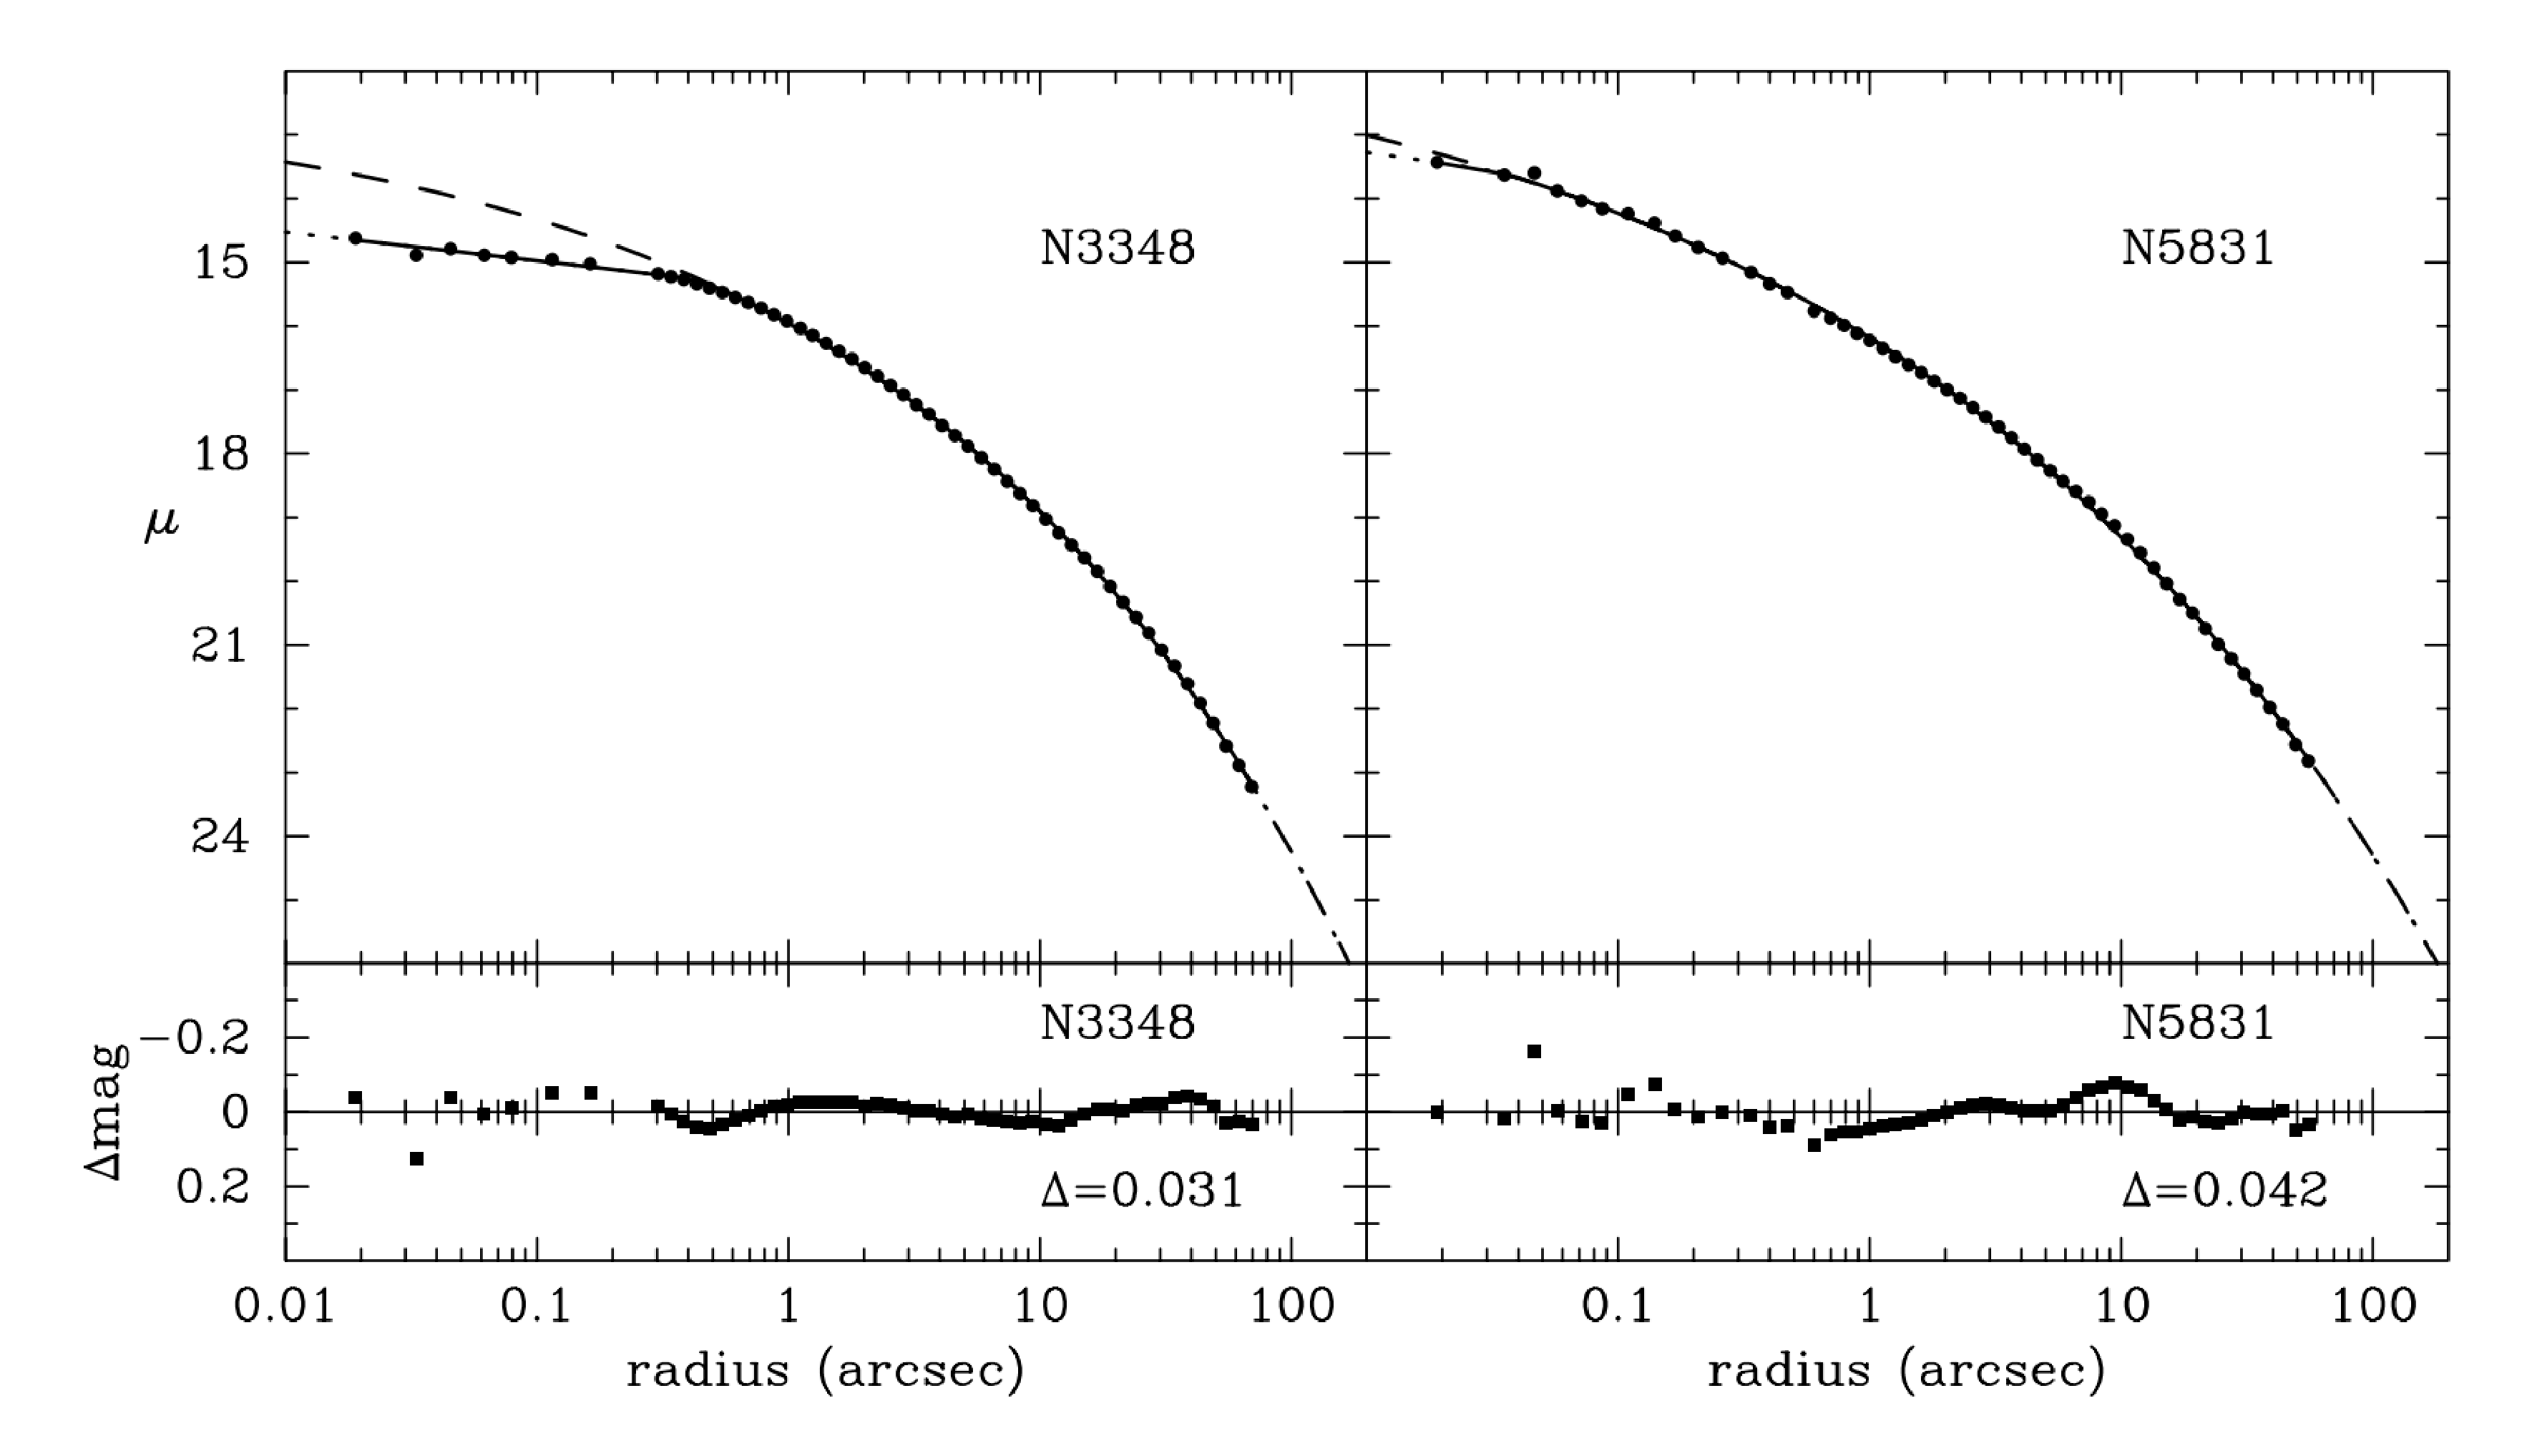
\includegraphics[width=0.9\textwidth]{images/sersiccoresersic.eps}
\end{center}
\caption{
The observed major-axis surface brightness radial profiles ($\mu$, in units of $\rm mag~arcsec^{-2}$) 
of the elliptical galaxies NGC 3348 and NGC 5831 
are shown with the black points in the top left and right panels, respectively. 
The solid lines are fits using the empirical core-S\'ersic model, 
and the dotted extensions are their inner and outer extrapolations. 
The long dashed lines indicate extrapolations of the outer S\'ersic-like part of the core-S\'ersic model. 
The residuals from the fits ($\Delta \mu = data - model$) are shown with black squares in the bottom panels, 
and the rms scatter $\Delta$ is given for each fit. 
This Figure was extracted from \cite{graham2003coresersicmodel}. }
\label{fig:corser}
\end{figure}

Partially depleted cores are believed to form during dissipationless (``dry'', i.e.~gas-poor) mergers \citep{begelman1980}, 
where the progenitor black holes sink towards the centre of the remnant galaxy due to dynamical friction against stars, 
form a bound pair and further reduce their orbital separation by transferring their binding energy to the surrounding stars 
via a three-body scattering process also known as ``gravitational slingshot'' 
(\citealt{milosavljevicmerritt2001,merritt2013CQG}, and references therein). 
The scouring action of the black hole binary has the effect of lowering the galaxy's stellar central density, 
in fact producing a partially depleted core 
(e.g.~\citealt{merritt2006RPP,dotti2012,colpi2014}). 
The lack of a significant amount of gas during the merger is a necessary condition 
to guarantee the formation of a partially depleted core. 
\cite{mayer2009} and \cite{colpi2009} followed the simulations of two merging Milky Way-like galaxies 
and reported that the time-scale for the formation of a close black hole binary system due to dynamical friction against gas 
is $\approx$100 times shorter than that due to dynamical friction against stars. 
Therefore, a black hole binary coalesces more quickly in a gas-rich (``wet'') merger than in a gas-poor (``dry'') merger, 
i.e.~when gas is in play, the binary does not have enough time to form a partially depleted core. 
In addition, gas is likely to be funnelled towards the centre of the galaxy remnant, shock and induce star formation, 
which would act against the formation of a core by increasing the central stellar density. 


\subsection{Origin of SMBHs}
As of today, the formation of SMBHs is still an unsolved puzzle. 
The key astrophysical questions that pertain to this open debate are: 
(\emph{i}) what are the initial seeds of SMBHs and when did they form? 
(\emph{ii}) how were these seeds distributed in the early universe 
(i.e.~what is their mass distribution function and space density)? 
and (\emph{iii}) what is their accretion history throughout the Universe's first few billion years? 
\cite{volonteribellovary2012} review three possible pathways -- not mutually exclusive -- 
that have been proposed as viable mechanisms to SMBH seeds formation. \\

The first of these three theoretical scenarios states that SMBHs originated from the remnants of Population III stars. 
Population III stars are the (hypothetical) first generation of stars, which formed out of zero-metallicity pristine gas. 
The lack of metals implies inefficient cooling and inefficient fragmentation of the gas, 
making possible to produce very massive stars (with initial masses $\gtrsim 100~\rm M_\odot$). 
The fate of Population III stars mainly depends on their initial mass \citep{heger2003}. 
A low-metallicity star that initially weights $\approx 25 - 140~\rm M_\odot$ is predicted to directly collapse into a black hole 
with about half of the mass of its progenitor star. 
Such black hole would not be heavy enough to be dragged by dynamical friction towards the host galaxy centre, 
therefore it would hardly contribute to the formation of a central SMBH. 
Between $\approx 140 - 260~\rm M_\odot$, low-metallicity stars lie within the pair instability supernova regime, 
where the final nuclear-powered explosion completely disrupts the star and leaves no remnant. 
Above $\approx 260~\rm M_\odot$, the nucleus of a low-metallicity star is highly unstable 
and quickly ($\approx 2~\rm Myr$) collapses into a black hole that retains at least half of the initial stellar mass. 
For many years, these high-mass stellar black holes have been considered the most promising SMBH seeds candidates. 
However, as recent numerical simulations were improved 
thanks to the achievement of better resolution and the inclusion of more complex physics 
(e.g.~\citealt{turk2009,greif2011,clark2011,stacy2012}), 
it became clear that fragmentation played a more important role in the formation of Population III stars, 
which turned into less attractive candidates for the origin of SMBHs. \\

A second possibility for the genesis of SMBH seeds is the formation of a supermassive star (up to $\approx 10^6~\rm M_\odot$) 
at the centre of a primordial galaxy. 
In this scenario, low-metallicity, low-angular momentum gas infalls towards the bottom of the potential well of a dark matter halo and, 
due to gravitational instabilities, does not settle into a rotationally supported disc, 
but accumulates into a very massive star, 
whose core rapidly ($\approx 1~\rm Myr$) collapses into a black hole and swallows the surrounding gas envelope, 
giving birth to a $\approx 10^3 - 10^6~\rm M_\odot$ SMBH seed. \\

According to the third theoretical scenario, gas infalls towards the centre of a dark matter halo and fragments into several stars
that form a dense stellar cluster. 
Before the first supernova explosions can occur, small stars collide with each other within the cluster 
and merge into a massive ($\approx 10^3~\rm M_\odot$) star which eventually collapses into a black hole with similar mass. \\

The discovery of ultraluminous quasars at $z>6$ has accentuated the urge to create very massive black hole seeds in a relatively short time 
(e.g.~\citealt{alexandernatarajan2014,madau2014,lupi2015}). 
To date, there have been nearly 50 claims of $z>6$ quasars hosting $\gtrsim 10^9~\rm M_\odot$ black holes 
(e.g.~\citealt{fan2003,jiang2007,mortlock2011,banados2014,trakhtenbrot2015,wu2015}). 
Within a $\Lambda$CDM cosmology, such early giant monsters could not have formed so quickly 
without the creation of anomalously massive seeds 
or incredibly high accretion rates, i.e.~exceeding the Eddington limit 
(but see \citealt{meliamcclintock2015} for an alternative explanation). 
However, it is worth noting that these black hole masses are calculated with the reverberation mapping method, 
assuming that $M_{\rm BH}$ is directly proportional to the virial factor $f$, 
which is calibrated on the normalisation of the $z=0$ observed $M_{\rm BH} - \sigma_*$ correlation. 
The existence of (unknown) selection biases in the local sample of directly measured black hole masses 
would imply a systematic overestimation of the virial factor and, consequently, 
of the black hole masses estimated with the reverberation mapping technique. \\


%\subsection{bhfp}
%\cite{marconihunt2003} pointed out a significant correlation between the residuals of the $M_{\rm BH} - \sigma_*$
%relation and the effective radii of the spheroids in their sample. 
%Motivated by this observation, many studies have explored the possibility that the different black hole mass 
%scaling relations were projections of the same black hole ``fundamental plane'' (BHFP), in analogy to the
%well known fundamental plane of spheroids ($R_{\rm e,sph} \propto \sigma_{*}^{\alpha} \langle \mu_{\rm e,sph}\rangle^{\beta}$,
%with $\langle \mu_{\rm e,sph}\rangle$ the mean bulge surface brightness within $R_{\rm e,sph}$, \citealt{djorgovskidavis1987}).
%Various three-parameter correlations have been investigated, in the form of $M_{\rm BH} - R_{\rm e,sph} - \langle \mu_{\rm e,sph}\rangle$ 
%\citep{barwaykembhavi2007}, 
%$M_{\rm BH} - R_{\rm e,sph} - \sigma_{*}$ \citep{marconihunt2003,defrancesco2006,allerrichstone2007,
%hopkins2007} and $M_{\rm BH} - R_{\rm e,sph} - n_{\rm sph}$ \citep{graham2008}.
%However, \cite{graham2008} revisited all the three versions of the BHFP and showed that none of them is defined by the population
%of barless spheroids. 
%In fact, the bulges of barred spiral galaxies systematically deviate from the $M_{\rm BH} - \sigma_*$ relation, 
%producing the apparent black hole plane. 
%\cite{graham2008} nevertheless pointed out that more and better quality data would be welcome in fully resolving this issue.
%
%
%This observation motivated \cite{hopkins2007} to search for a black hole ``fundamental plane'' (BHFP), in analogy to the
%well known fundamental plane of spheroids ($R_{\rm e} \propto \sigma_{*}^{\alpha} I_{\rm e}^{\beta}$).
%They found that the systems in their sample lie on a BHFP of the form $M_{\rm BH} \propto \sigma_{*}^{3.0} R_{\rm e}^{0.5}$ 
%or $M_{\rm BH} \propto M_{*}^{0.5 - 0.7} \sigma_{*}^{1.5 - 2.0 }$.


%\subsection{fundamental corr}

\subsection{Monster black holes}
\label{sec:monsters}
Over the last five years, several claims of detections of \emph{over-massive} black holes accumulated in the literature. 
Over-massive black holes are black holes whose mass is significantly larger 
than what is expected from the galaxy's spheroid stellar velocity dispersion or stellar mass, 
i.e.~they are positive outliers in the $M_{\rm BH} - \sigma_*$ or $M_{\rm BH} - M_{\rm *,sph}$ diagrams. \\

Using integral-field spectrographs at the Gemini North and Keck 2 telescopes, 
\cite{mcconnell2011} targeted the BCGs (NGC 3842 and NGC 4889) of two massive galaxy clusters, 
the Leo and Coma clusters (Abell 1367 and Abell 1656, respectively), 
and reported the direct detection of the two most massive black holes ever found at that time. 
They claimed that these two black holes are significantly more massive 
than predicted by the popular $M_{\rm BH} - \sigma_*$ and $M_{\rm BH} - L_{\rm sph}$ correlations, 
and speculated that the growth of the largest galaxies and their black holes happens by means of evolutionary processes 
different from what is commonly assumed for less massive elliptical galaxies. \\

\cite{rusli2011} obtained SINFONI integral-field unit observations of the nuclear region of the galaxy NGC 1332 
and measured a one billion solar masses black hole, 
consistent with the galaxy's stellar velocity dispersion, 
but offset from the $M_{\rm BH} - L_{\rm sph}$ relation by a full order of magnitude. \\

\cite{vandenbosch2012} combined archival Hubble Space Telescope (\emph{HST}) high-resolution imaging 
and long-slit spectroscopy (obtained with the Marcario Low Resolution Spectrograph on the Hobby-Eberly Telescope, Texas) 
of the nuclear region of the galaxy NGC 1277, 
and directly measured the central black hole mass by fitting self-consistent Schwarzschild models 
to the integrated stellar kinematics. 
They found a twenty billion solar masses black hole, 
which they estimated to weight 59\% of the host spheroid's mass (or 14\% of the galaxy's total stellar mass). 
According to their measurement, 
the black hole of NGC 1277 was an order of magnitude more massive than what expected from the host spheroid's stellar velocity dispersion 
and two orders of magnitude more massive than what expected from the host spheroid's stellar mass.
\cite{emsellem2013} re-analysed \citeauthor{vandenbosch2012}'s data 
and showed that their observations were consistent with a black hole mass up to an order of magnitude smaller 
than the extraordinary value previously reported. 
However, \cite{yildirim2015} and \cite{scharwachter2015} confirmed \citeauthor{vandenbosch2012}'s measurement. \\

\cite{bogdan2012} reported on the unusually high $M_{\rm BH}/M_{*,sph}$ ratio for the galaxies NGC 4342 and NGC 4291 
and concluded that no co-evolution subsisted between these two galaxies and their black holes. 
Other reportedly over-massive black holes belong to the galaxies NGC 1271 \citep{walsh2015} and Mrk 1216 \citep{yildirim2015}. \\

On the basis of these claims, \cite{ferremateu2015} theorised that, 
while most today's massive early-type galaxies have completed their two-phase growth path (``in-situ'' and ``ex-situ''), 
the over-massive black holes hosts skipped the second (``ex-situ'') phase and therefore represent an exception. 


\section{Galaxy decomposition}
Galaxy decomposition is a parametric analysis that allows one to fit the surface brightness distribution
of galaxies using a combination of analytic functions (usually one function per
galaxy component, such as spheroid, disc, bar, nucleus, etc.). 
The 1D (one-dimensional) technique begins with fitting isophotes to the galaxy image.
Isophotes are curves along which the intensity of light is constant 
and they are typically described with concentric ellipses.  
The 1D surface brightness radial profile is then extracted and modelled with a combination of 1D analytic functions. 
With the 2D (two-dimensional) technique one fits 2D analytic functions directly to digital images. 
Galaxy decomposition is useful to perform structural analysis of galaxies and obtain the best-fit 
parameters of the spheroidal component, such as the luminosity, the half-light radius 
and the central radial concentration of stars. \\

\begin{figure}[htb]
\begin{center}
\includegraphics[width=\textwidth]{images/galaxyvivisection.eps}
\end{center}
\caption{Schematic representation of one-dimensional galaxy decomposition. 
The mock galaxy at the top is composed of a spheroid (orange), a large-scale disc (blue), 
a bar (green), and a nuclear source (red). 
The observed surface brightness profile of the galaxy (intensity of light as a function of galactocentric radius) 
is the white curve. 
The contribution of each galaxy component to the total surface brightness profile is modelled with one analytic function, 
illustrated with a solid line of the same colour as the corresponding component. 
The sum of all analytic functions gives the total galaxy model, 
which is matched to the observed surface brightness profile. }
\end{figure}

Pioneer studies that performed 1D bulge/disc decompositions of galaxies (e.g.~\citealt{simiendevaucouleurs1986}) 
described the bulge component with a \cite{devaucouleurs1948} $R^{1/4}$ profile:
\begin{equation}
\mu_{\rm de Vaucouleurs}(\mu_{\rm e},R_{\rm e};R) = \mu_{\rm e} + 8.32678
\Biggl[\biggl(\frac{R}{R_{\rm e}}\biggr)^{1/4}-1\Biggr] ,
\end{equation} 
and the disc component with an exponential profile:
\begin{equation}
\mu_{\rm exponential}(\mu_{\rm 0},h;R) = \mu_{\rm 0} + \frac{2.5}{\ln(10)} \biggl(\frac{R}{h} \biggr) .
\end{equation} 
Here $\mu$ is the surface brightness profile, 
$R$ is the projected galactic radius, i.e.~the distance of the isophotes from the galaxy centre, 
$R_{\rm e}$ is the bulge effective radius (or half-light radius) that encloses half of the total light from the model, 
$\mu_{\rm e}$ is the bulge surface brightness at the effective radius, 
$\mu_{\rm 0}$ is the disc central surface brightness, 
and $h$ is the disc scale length. \\

However, it soon became clear to some that the fixed curvature of the two-parameter de Vaucouleurs $R^{1/4}$ law 
was not adequate to accommodate the variety of shapes observed in the light profiles of stellar spheroidal systems. 
A more ductile mathematical function was needed 
such as the three-parameter \cite{sersic1963,sersic1968} $R^{1/n}$ model: 
\begin{equation}
\mu_{\rm S\acute{e}rsic}(\mu_{\rm e},R_{\rm e},n;R) = \mu_{\rm e} + \frac{2.5~b_{\rm n}}{\ln(10)} 
\Biggl[\biggl(\frac{R}{R_{\rm e}}\biggr)^{1/n}-1\Biggr] ,
\end{equation}
where the S\'ersic index $n$ is the parameter that measures the curvature of the radial light profile,
and $b_{\rm n}$ is a scalar value defined in terms of the S\'ersic index 
(see \citealt{grahamdriver2005} for a valuable compendium). 
After \cite{caon1993} and \cite{donofrio1994} demonstrated the superiority of the S\'ersic model 
over the de Vaucouleurs law in describing the spatial distribution of light of early-type galaxies, 
the varying curvature of the S\'ersic model became a necessity also for rendering 
the light profiles of the bulges of spiral galaxies 
\citep{andredakis1995,moriondo1998,grahamprieto1999,khosroshahi2000,graham2001}. \\

Thanks to the improved computational speed of machines, 
2D fitting algorithms have become more and more popular over the last two decades. 
\cite{dejong1996} presented a 2D decomposition technique 
which allowed one to model the surface photometry of a galaxy 
using an exponential light profile for both the bulge and the disc. 
\cite{simard1998} developed the IRAF\footnote{IRAF is the Image Reduction and Analysis Facility, 
distributed by the National Optical Astronomy Observatory, 
which is operated by the Association of Universities for Research in Astronomy (AURA) 
under cooperative agreement with the National Science Foundation.} package {\tt GIM2D}, 
a 2D decomposition code aimed at distant galaxies. 
{\tt GIM2D} takes an input image and simultaneously decomposes all the objects 
as the sum of a S\'ersic and an exponential profile. \\

A major breakthrough came with {\tt GALFIT}, 
a 2D fitting algorithm released by \citeauthor{peng2002} (\citeyear{peng2002}; 
the nowadays popular {\tt GALFIT3}, an improved version of the original algorithm, was presented by \citealt{peng2010}), 
which marked an important turning point for the quantitative morphological analysis of galaxies. 
Thanks to its capability of fitting a galaxy with an arbitrary number of components 
-- chosen from a wide variety of analytical functions such as the S\'ersic and the ``Nuker'' models, 
or the exponential, Gaussian, and Moffat profiles -- 
and to its optimisation in computational speed, 
{\tt GALFIT} was specifically conceived for modelling large images of spatially well-resolved, 
nearby galaxies observed with the Hubble Space Telescope. \\

\cite{desouza2004} developed {\tt BUDDA} (Bulge/disc Decomposition Analysis), 
a code to perform 2D decomposition of galaxies using a two-component S\'ersic+exponential model. 
The number of fitted components was intentionally limited to two (bulge+disc), 
with the purpose of using the residual images 
to study the additional substructures such as bars, lenses, rings, and inner discs. \\

\cite{laurikainen2005} opted for a hybrid approach, 
combining the advantages of a 2D decomposition technique 
with the insight gained from a 1D isophotal analysis. 
In this exemplary study, the authors modelled the images of 24 early-type disc galaxies (S0/S0a) 
accounting for bulge, disc, bars, ovals/lenses\footnote{According to their nomenclature, 
an egg-shaped structure (with axis ratio $b/a \gtrsim 0.85$) 
embedded within the large-scale disc of a galaxy 
is dubbed lens or oval in case of a lenticular or spiral galaxy, respectively. 
Lenses/ovals and pseudobulges might have similar ellipticities, 
but the former typically have lower surface brightness and sharper outer edges than the latter 
\citep{kormendykennicutt2004}. }, and inner discs. 
Their decomposition method was assessed on synthetic images of galaxies composed of a bulge, 
a large-scale disc, and a bar. 
They tested the effects of the omission of the bar component from the galaxy model. 
While a three-component (bulge+disc+bar) model was correctly recovering the real bulge parameters, 
a two-component (bulge+disc) model was overestimating the bulge luminosity by up to 40\% 
because the S\'ersic model for the bulge was somehow ``forced'' to account also for the bar. 
They also experimented with a large number of different weighting maps, 
and concluded that the results from the fit were not significantly dependent on the choice of the weighting function,
unless the signal-to-noise of the galaxy image was extremely low, 
or a prominent component was not included in the model. 
In addition, they pointed out that a fit lacking seeing correction resulted in notably biased bulge parameters. 
\cite{laurikainen2005} stressed an important point about galaxy decomposition: 
in order to have control of the physical meaning of the different components in a galaxy, 
\emph{a priori} evaluation of the existence of such components is required. 
This concept is opposed to the (nowadays popular) approach of repeating the fit of a galaxy 
by continuously increasing the number of model components 
until all residual structures are eliminated from the residual image.  
\cite{laurikainen2005} used three different methods to identify the structural components of a galaxy:
they inspected (\emph{i}) the radial profiles of ellipticity and position angle of the galaxy's isophotes, 
whose bumps often correspond to bars, ovals/lenses, and inner discs 
when these components are sufficiently bright compared to the large-scale disc, 
(\emph{ii}) the radial profiles of low azimuthal wavenumber Fourier amplitudes and phases, 
sensitive to weak bars and ovals/lenses, 
and (\emph{iii}) the unsharp masks\footnote{Unsharp masks are obtained from the original images 
with a mathematical operation of convolution. By suppressing large-scale, low-frequency variations 
in the images, they act as a filter and reveal faint asymmetric structures within the galaxies 
\citep{malinzealey1979,erwinsparke2003}.}, useful to reveal the innermost structures. 
Upon comparing the results from their three-component decompositions 
with those obtained from the two-component decompositions of \cite{simiendevaucouleurs1986} in the B-band 
and \cite{desouza2004} in the K$_S$-band, 
\cite{laurikainen2005} noted that their bulge-to-total ratios were considerably smaller for all Hubble types. 
This large discrepancy was not due to the wavelength used, 
but to the fact that, when a galaxy model does not account for a bar, 
a large fraction of the bar light erroneously goes into the bulge model, 
artificially increasing the bulge-to-total ratio. 
This sophisticated decomposition method was applied to the analysis of 175 early-type disc galaxies 
using deep near-infrared imaging \citep{laurikainen2007,laurikainen2010},  
and the results from these decompositions were used for a detailed study of bars, ovals/lenses and bulges. 
They found ovals/lenses in 70\% of the S0/S0a galaxy sample, 
and nuclear components (bars/rings/discs) in 50\% of them. 



\subsection{Photometry and kinematics}
\label{sec:photokin}
Early-type galaxies can exhibit a wide variety of kinematic features, 
going from the fainter rotationally-supported systems to the brighter dispersion-dominated ones (e.g.~\citealt{davies1983}). 
While the identification of stellar discs in images of spiral galaxies is generally trivial thanks to the presence of spiral arms, 
featureless discs in bright, early-type galaxies can be particularly hard to recognise 
by looking at the photometry alone, due to well-known inclination effects (e.g.\citealt{rixwhite1990,gerhardbinney1996}). 
However, this problem can be alleviated with the use of kinematic information
(e.g.~\citealt{carter1987,franx1989,nieto1991,rixwhite1992,cinzanovandermarel1993,donofrio1995,graham1998fornax}).
In particular, our understanding of the internal structure of early-type galaxies has undoubtedly improved over the past decade 
thanks to the introduction of integral-field spectrographs and the analysis of two-dimensional kinematic maps 
(e.g.~the ATLAS$^{\rm 3D}$ survey, \citealt{cappellari2011}). \\

\cite{emsellem2007} used the specific angular momentum within one effective radius 
($\lambda_{\rm R} = \langle R |V| \rangle / \langle R \sqrt{V^2 + \sigma^2} \rangle $, 
where $R$ is the semimajor-axis radius, $V$ is the mean velocity and $\sigma$ is the velocity dispersion)  
and the ellipticity at one effective radius 
($\epsilon = 1 - (b/a)$, 
where $(b/a)$ is the ratio of minor-to-major axis length) 
to classify early-type galaxies into fast rotators and slow rotators, 
based on the empirical divide $\lambda_{\rm R} = 0.31 \sqrt{\epsilon}$. \\

\cite{krajnovic2006} developed ``kinemetry'', 
a method that combines surface photometry and kinematics 
to recognise less obvious structures in galaxies, such as embedded discs and kinematic subcomponents. 
Using kinemetry, \cite{krajnovic2011} measured the regularity of velocity maps 
and demonstrated that fast rotators are typically nearly axisymmetric systems, 
whereas most slow rotators are triaxial systems. 
At present, the joint effort of imaging and integral-field spectroscopy is undeniably our best chance 
to disclose the internal structure of galaxies (e.g.~\citealt{krajnovic2015IAUS}).  \\

Putting this paradigm into practice, 
\cite{krajnovic2013} compared photometric signatures and kinematic properties of stellar discs 
for the 180 unbarred early-type galaxies of the ATLAS$^{\rm 3D}$ sample. 
For each galaxy, they fit the light distribution using a single bulge \citep{sersic1963,sersic1968} 
and a bulge+disc (S\'ersic+exponential) model, 
preferring the latter when the improvement over the single bulge model was substantial 
and no correlation within the residuals was observed. 
They found that exponential sub-components in fast rotators correspond 
to a genuine family of rotationally-supported discs or disc-like structures, 
which were identified in 83\% of the unbarred early-type subsample,
contributing to 40\% of the total stellar mass and  
covering a full range of disc-to-total flux ratios. 
From their analysis, \cite{krajnovic2013} concluded that, when using photometry only, 
inclination effects do not particularly affect the identification of dominant discs, 
but they become much more disruptive when dealing with low-inclination, medium size discs. 
The use of kinematics is therefore the best approach to mitigate inclination effects. 
One of the key results obtained by the ATLAS$^{\rm 3D}$ Collaboration is that 
the majority of early-type galaxies contain stellar discs 
with an essentially continuous distribution of disc-to-total flux ratios, 
which led \cite{cappellari2011} to the introduction of a new classification scheme 
aimed at replacing the classical Hubble diagram. \\



\subsection{A compendium of the previous literature }
Over the past nine years, five independent studies 
\citep{grahamdriver2007,sani2011,vika2012,beifiori2012,lasker2014data,lasker2014anal}
have attempted galaxy decomposition 
for samples of galaxies with a direct measure of the black hole mass. 
The main aim of each study was to derive the parameters of the spheroidal components of their galaxies 
and explore correlation with the black hole mass.
Table \ref{tab:lit} summarises the main characteristics and findings of each work. 
%The last column refers to the study presented in this thesis 
%and highlights its improvements over the past literature.

\begin{table}[ht] 
\footnotesize
%\small
\centering 
\begin{tabular}{llllll}
\hline\hline 
		       & {\bf GD07}	 & {\bf S+11}	   & {\bf V+12} & {\bf B+12}  & {\bf L+14} \\ 	      %& {\bf This work}   \\ 
\hline \\ [-1.5ex]
{\bf Galaxies }        & 27		 & 57		   & 25 	& 19	      & 35	   \\	      %& 66		  \\
{\bf Wavelength }      & R-band 	 & $3.6~\mu \rm m$ & K-band	& $i$-band    & K-band     \\	      %& $3.6~\mu \rm m$   \\
{\bf Decomposition}    & 1D		 & 2D		   & 2D 	& 2D	      & 2D	   \\	      %& 1D \& 2D	  \\
{\bf Nuclei }	       & masked 	 & modelled	   & modelled	& not treated & modelled    \\	      %& modelled/masked    \\
{\bf Cores }	       & masked 	 & masked	   & masked	& not treated & masked     \\ 	      %& masked  	  \\ 
{\bf Bars }	       & excluded	 & modelled	   & modelled	& excluded    & modelled    \\ 	      %& modelled 	  \\ 
{\bf Other components} & no		 & no		   & no 	& no	      & yes	   \\ 	      %& yes		  \\ 
{\bf Kinematics}       & no		 & no		   & no 	& no	      & no	   \\ [0.5ex] %& yes		  \\ [0.5ex] 
\hline
\multicolumn{6}{c}{\emph{Conclusions}} \\ 
\hline \\ [-1.5ex]
$\boldsymbol{ M_{\rm BH}-n_{\rm sph}}$  		& yes	& no	     & no  & no        & -	     \\ 	%& -   \\
$\boldsymbol{ M_{\rm BH}-L_{\rm sph}}$  		& -	& yes	     & yes & yes       & fundamental \\ 	%& -   \\
$\boldsymbol{ M_{\rm BH}-M_{\rm sph,dyn}}$		& -	& yes	     & -   & yes       & -	     \\ 	%& -   \\
$\boldsymbol{ M_{\rm BH}-M_{\rm sph,*}}$		& -	& yes	     & -   & -         & -	     \\ 	%& -   \\
$\boldsymbol{ M_{\rm BH}-R_{\rm e}}$			& -	& secondary  & -   & -         & -	     \\ 	%& -   \\
$\boldsymbol{ M_{\rm BH}-\langle \mu_{\rm e} \rangle}$  & -	& -	     & -   & no        & -	     \\ 	%& -   \\
$\boldsymbol{ M_{\rm BH}-L_{\rm gal}}$  		& -	& -	     & -   & secondary & fundamental \\ [0.5ex] %& -   \\ [0.5ex] 
\hline 
\hline 
\end{tabular}
\caption{ Main characteristics and findings of the latest five studies that have attempted galaxy decomposition 
to derive and explore black hole mass scaling relations. 
The number of galaxies accounts only for those with a direct measurement of the black hole mass 
(no upper limits are considered here). 
GD07 = \cite{grahamdriver2007}; S+11 = \cite{sani2011}; V+12 = \cite{vika2012}; B+12 = \cite{beifiori2012}; 
L+14 = \cite{lasker2014data,lasker2014anal}.}
\label{tab:lit} 
\end{table}

\cite{sani2011} used galaxy images 
obtained with the \emph{Spitzer} satellite in the $3.6~\mu \rm m$ wavelength-band, 
which currently represents the best proxy for the stellar mass, 
even superior to the K-band (\citealt{sheth2010}, and references therein). \\

%Besides using the largest sample of galaxies to date, 
%this work is based on observations in the $3.6~\mu \rm m$ wavelength-band, obtained with the \emph{Spitzer} satellite,
%which currently represents the best proxy for the stellar mass (\citealt{sheth2010}, and references therein). 
There has been an ongoing debate as to whether 2D galaxy decomposition techniques should be preferred over 1D techniques. 
The performance of each method can vary according to different technical factors 
(such as the signal-to-noise of the galaxy images, the accuracy of the description of the Point Spread Function, 
the gradient of ellipticity and position angle of the galaxy isophotes, 
the fitting weighting scheme, etc.), 
therefore advantages and disadvantages are not absolute and depend on the individual science case. 
To our best knowledge, 
no published study has ever been conducted on a systematic comparison between 1D and 2D galaxy decomposition techniques. \\

%we chose to experiment with both methods and compare the results. 
Previous works have demonstrated that, when studying galaxies with a complex morphology, 
the accuracy of the recovery of the bulge parameters increases 
when all galaxy components are taken into account by the model  
\citep{laurikainen2005,gadotti2008,salo2015}. 
\cite{lasker2014data} identified and modelled more galaxy components than any other study,
but no work did it with the assistance of kinematical information. \\

Interestingly, the past studies all used almost the same sample of galaxies 
(the number of directly measured black hole masses increased with time), 
but they claimed some contradictory conclusions. 
One study obtained a good $M_{\rm BH}-n_{\rm sph}$ correlation, whereas three did not.
\cite{lasker2014anal} elected the $M_{\rm BH}-L_{\rm gal}$ relation as the fundamental one
(likewise the $M_{\rm BH}-L_{\rm sph}$), 
as opposed to \cite{beifiori2012}, who presented it as a secondary correlation.
The past studies did not converge to the same conclusions 
because their best-fit models for the same galaxy were often 
significantly different and not consistent with each other in terms 
of fitted components. 
Moreover, none of these studies attempted an individual galaxy-by-galaxy 
comparison of their models with the previous literature. 
%We have now made this comparison, identified the optimal decomposition, 
%and obtained improved black hole mass scaling relations using a large sample of galaxies.
%Our work will also present a comparison between 1D and 2D galaxy decompositions.

\section{Thesis outline}
The aim of this thesis is to refine and re-investigate several black hole mass scaling relations 
through the careful modelling of the spatial light distribution 
of a selected sample of 66 nearby galaxies. 
After obtaining robust structural parameters for the galaxies under study, 
I will explore substructure in the correlations between these parameters and the black hole mass, 
and explain discrepancies in the results presented in the past literature. \\

In Chapter \ref{ch:recov-mn} \citep{savorgnan2013}, 
we tackle the issue of the $M_{\rm BH} - n_{\rm sph}$ correlation using literature data. 
Four studies independently carried out photometric decompositions for similar samples of galaxies, 
but only one of them obtained a statistically significant $M_{\rm BH} - n_{\rm sph}$ relation. 
For each galaxy analysed by two or more studies, 
we compared the models used to fit the galaxy's spatial distribution of light, 
and found that the same galaxy was often described with remarkably different models 
in terms of number and type of sub-components. 
This was obviously resulting in significantly different best-fit parameters. 
We then collected the S\'ersic index measurements obtained by the four studies for 54 common galaxies 
with a direct measure of their black hole mass, 
rejected the most discrepant values, 
and used the remaining measurements to populate the $M_{\rm BH} - n_{\rm sph}$ diagram. 
Besides recovering a statistically significant $M_{\rm BH} - n_{\rm sph}$ relation for all galaxies, 
we also explored substructure for different galaxy morphological types 
(elliptical galaxies versus bulges of disc galaxies)
and nature of the nuclear light profile (S\'ersic versus core-S\'ersic). \\

In Chapter \ref{ch:galviv} \citep{paperI}, 
we present the 1D decompositions carried out by us for 66 local galaxies 
with a direct measure of their black hole mass. 
We describe the careful data reduction process through which 
we created the image-mosaics for these galaxies, 
using archival observations at $3.6~\mu \rm m$ obtained with \emph{Spitzer}. 
We detail our 1D galaxy decomposition technique and our method to estimate the uncertainties 
associated with the spheroid's best-fit parameters. 
Upon comparing the results obtained from our 1D and 2D galaxy models, 
we comment on the advantages and disadvantages connected with 1D and 2D decomposition techniques. 
The individual 1D galaxy decompositions are illustrated, 
along with a thorough analysis of each galaxy's structure 
and a scrupulous comparison with several past decompositions. \\
 
In Chapter \ref{ch:mm} \citep{paperII}, 
we use the results from our 1D galaxy decompositions 
to explore substructure in the $M_{\rm BH} - L_{\rm gal}$ and $M_{\rm BH} - L_{\rm sph}$ 
(or $M_{\rm BH} - M_{\rm *,sph}$) diagrams 
for different galaxy morphological types and nature of the nuclear light profile. 
Upon performing a detailed linear regression analysis using three different routines, 
we concluded that early-type (elliptical+lenticular) and late-type (spiral) galaxies 
follow two separate correlations in the $M_{\rm BH} - L_{\rm sph}$ (or $M_{\rm BH} - M_{\rm *,sph}$) diagram. 
In addition, we compared the level of intrinsic scatter 
in the $M_{\rm BH} - L_{\rm gal}$ and $M_{\rm BH} - L_{\rm sph}$ diagrams 
to address the question of whether or not the $M_{\rm BH} - L_{\rm sph}$ correlation 
is more fundamental than the $M_{\rm BH} - L_{\rm gal}$ correlation. \\

In Chapter \ref{ch:mn} \citep{paperIII}, 
we use the results from our 1D galaxy decompositions to populate 
the $L_{\rm sph} - n_{\rm sph}$ and $M_{\rm BH} - n_{\rm sph}$ diagrams. 
The analysis that we performed here is essentially analogous to that presented in Chapter \ref{ch:mm}.  
We did not observe any significant substructure in the $M_{\rm BH} - n_{\rm sph}$ diagram, 
where all galaxies, irrespective of their morphological type, define a single tight correlation. 
Consistency between the $M_{\rm BH} - n_{\rm sph}$ and other galaxy scaling relations 
is dicussed here.  \\

In Chapter \ref{ch:msigma} \citep{savorgnangraham2015}, 
we concentrate on the $M_{\rm BH} - \sigma_*$ scaling relation 
and the presence of some outlying, ``overmassive'' black holes at the high-mass end of this correlation. 
\cite{volontericiotti2013} proposed a theoretical interpretation 
to explain why central cluster galaxies tend to appear as positive outliers 
in the $M_{\rm BH} - \sigma_*$ diagram, lying above the observed $z=0$ correlation. 
According to the results from their semi-analytical models, 
central cluster galaxies experienced more dry mergers 
than the ``average'' population of massive early-type galaxies. 
Dry mergers are expected to increase the black hole mass, 
while leaving almost unchanged the stellar velocity dispersion. 
We tested the interpretation offered by \cite{volontericiotti2013} 
using the latest observational data. 
First, we updated the $M_{\rm BH} - \sigma_*$ diagram with a total of 89 galaxies 
and performed a linear regression analysis of it. 
Then, for each galaxy with a parially depleted core 
we measured the extent of dry mergers experienced by the galaxy 
by means of the ratio between the central stellar mass deficit and the black hole mass. 
We showed that no positive trend is observed between the number of dry mergers 
and the positive vertical offset from the $M_{\rm BH} - \sigma_*$ correlation. 
A similar test using the kinematics of galaxies gave consistent results, 
disproving the scenario advocated by \cite{volontericiotti2013}. \\

In Chapter \ref{ch:ellic} \citep{ellicular}, 
we tackle the issue of the ``overmassive'' black holes 
in the $M_{\rm BH} - M_{\rm *,sph}$ diagram. 
Due to inaccurate decompositions that failed to take into account the correct size of the main disc component, 
a number of galaxies (Mrk 1216, NGC 1271, NGC 1277, and NGC 1332) had their spheroid luminosity underestimated, 
which made them appear as positive outliers above the $M_{\rm BH} - M_{\rm *,sph}$ correlation. 
With the aid of photometric and kinematic information, 
we identified the radial extent of the main disc component, 
and built a galaxy model accordingly. 
We showed that when these galaxies are correctly modelled, 
they lie well within the scatter of the observed $M_{\rm BH} - M_{\rm *,sph}$ correlation. \\

Finally, Chapter \ref{ch:concl} contains a summary of my principal findings, conclusions, 
and some promising directions for future research. 
